\section{Introduction}
\label{sec:intro}

Videos are 2D projections of an evolving 3D world, where the underlying generative factors consist of spatial variation (camera viewpoint) and temporal evolution (dynamic scene motion). Learning to understand and disentangle these factors from observed videos is fundamental for tasks such as scene understanding, 4D reconstruction, video editing, and generative rendering, to name a few.  In this work, we approach this challenge from the perspective of generative rendering. Given a single observed video of a dynamic scene, our goal is to synthesize novel views (reframe/reangle) and/or at different moments in time (retime), while remaining faithful to the underlying scene dynamic. 

A common strategy is to first reconstruct dynamic 3D content from 2D observations, \ie, perform 4D reconstruction, and then re-render the scene. 
These methods model both spatial and temporal variations using representations such as NeRFs \cite{lin2024dynamic,mildenhall2021nerf} or Dynamic Gaussian Splatting \cite{kerbl20233d,wu20244d}, often aided by cues like geometry \cite{park2021hypernerf,park2021nerfies}, optical flow \cite{li2023dynibar,li2021nsff}, depth \cite{gao2021dynamic,yoon2020novel}, or long-term 2D tracks \cite{wang2024shapeofmotion,lei2024mosca}. However, even full 4D reconstructions typically show artifacts under novel viewpoints.
More recent work \cite{Wu2024, liang2024diffusion4d} uses multi-view video diffusion to generate sparse, time-conditioned views and refines them via Gaussian-splatting optimization, but rendering quality remains limited.
Advances in video diffusion models \cite{zhang2024show, wang2024lavie, blattmann2023stable, jeong2024track4gen, bar2024lumiere, videoworldsimulators2024, yang2024cogvideox, polyak2024moviegencastmedia, kong2024hunyuanvideo} further enable camera re-posing with more lightweight point cloud representations, reducing the need for heavy 4D reconstruction. While effective in preserving identity, their reliance on per-frame depth and reprojection limits robustness under large viewpoint changes. To mitigate this, newer approaches condition generation solely on camera parameters, achieving strong novel-view synthesis on both static \cite{jin2025lvsm} and dynamic scenes \cite{Bai2025,vanhoorick2024gcd,He2025}. 
Autoregressive models like Genie-3 \cite{parker-holder2025genie3} even enable interactive scene exploration from a single image, showing that diffusion models can encode implicit 4D priors. 
Nonetheless, despite progress in spatial viewpoint control, current methods still lack full 4D exploration, \ie, the ability to navigate scenes freely across both space and time.

\begin{figure}[t]
    \centering
    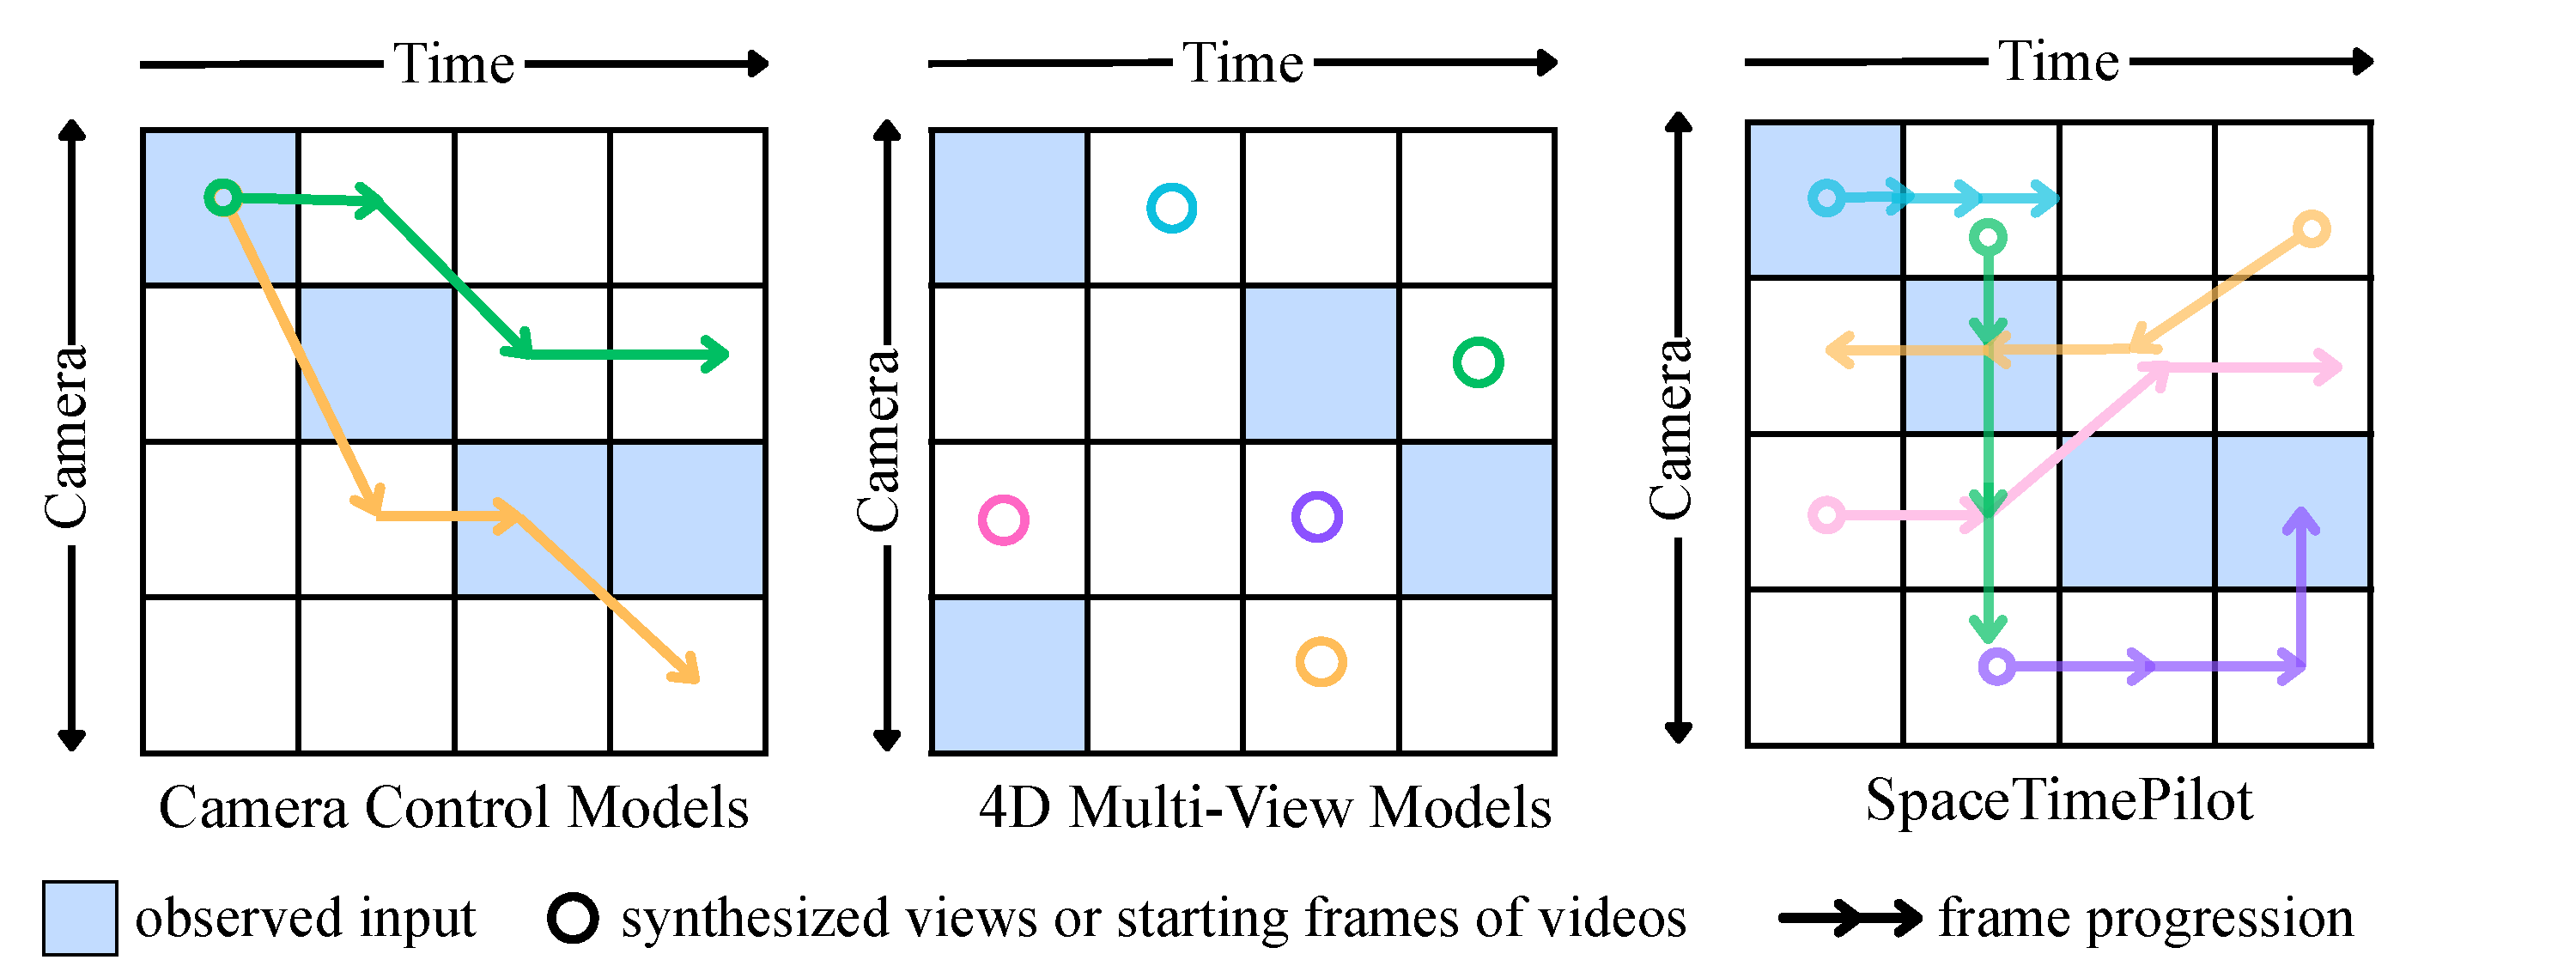
\includegraphics[width=\linewidth]{figures/src_files/high-level-concept.pdf}

\caption{\textbf{Space–time controllability across methods.}
Blue cells denote the input video/views, while arrows and dots indicate generated continuous videos or sparse frames. 
Camera-control V2V models~\cite{Bai2025, vanhoorick2024gcd} modify only the camera trajectory while keeping time strictly monotonic. 
4D multi-view models~\cite{Wu2024, liang2024diffusion4d} synthesize discrete sparse views conditioned on space and time, but do not generate continuous video sequences. 
\textit{SpaceTimePilot} enables free movement along both the camera and time axes with full control over direction and speed, supporting bullet-time, slow-motion, reverse playback, and mixed space–time trajectories.}

    \label{fig:high_level}
    \vspace{-3mm}
\end{figure}

In this work, we introduce \textit{\nameMethod}, the first video diffusion model that enables joint spatial and temporal control. \nameMethod introduces a new notion of ``animation time'' to capture the \textit{temporal status} of scene dynamics in the source video. As such, it naturally disentangles temporal control and camera control by expressing them as two independent signals. 
A high-level comparison between our approach and prior methods is illustrated in Fig.~\ref{fig:high_level}. Unlike previous methods, \nameMethod enables free navigation along both the camera and time axes.
Training such a model requires dynamic videos that exhibit multiple forms of temporal playback while simultaneously being captured under multiple camera motions, which is only feasible in a controlled studio setups. 
Although temporal diversity can be increased by combining multiple real datasets \eg \cite{zhou2018stereo,ling2024dl3dv}, as done in \cite{watson2025controllingspacetimediffusion,Wu2024}, this approach remains suboptimal, as the coverage of temporal variation is still insufficient to learn the underlying meaning of temporal control.
Existing synthetic datasets \cite{Bai2025, bai2024syncammaster} also do not exhibit such properties.

To address this limitation, we introduce a simple yet effective \textit{temporal-warping training scheme} that augments existing multi-view video datasets \cite{Bai2025, bai2024syncammaster} to simulate diverse conditioning types while preserving continuous video structure. By warping input sequences in time, the model is exposed to varied temporal behaviors without requiring additional data collection. This simple yet crucial strategy allows the model to learn temporal control signals, enabling it to directly exhibit space–time disentanglement effects during generation.
We further ablate various temporal-conditioning schemes and introduce a convolution-based temporal-control mechanism that enables finer-grained manipulation of temporal behavior and supports effects such as bullet-time at any timestep within the video.
While temporal warping increases temporal diversity, it can still entangle camera and scene dynamics -- for example, temporal manipulation may inadvertently affect camera behavior. 
To further strengthen disentanglement, we introduce a new dataset that spans the full grid of camera–time combinations along a trajectory. Our synthetic \textit{\nameDataset} dataset contains 180k videos rendered from 500 animations across 100 scenes and three camera paths. Each path provides full-motion sequences for every camera pose, yielding dense multi-view and full-temporal coverage. This rich supervision enables effective disentanglement of spatial and temporal control.

Experimental results show that \nameMethod successfully disentangles space and time in generative rendering from single videos, outperforming adapted state-of-the-art baselines by a significant margin. 
Our main contributions are summarized as follows:
\begin{itemize}
\item	We introduce \nameMethod, the first video diffusion model that disentangles spatial and temporal factors to enable continuous and controllable novel view synthesis as well as temporal control from a single video.
\item  We propose the \textit{temporal-warping strategy} that repurposes multi-view datasets to simulate diverse temporal variations. By training on these warped sequences, the model effectively learns temporal control without the need for explicitly constructed video pairs captured under different temporal settings.
\item	We propose a more precise camera–time conditioning mechanism, illustrating how viewpoint and temporal embeddings can be jointly integrated into diffusion models to achieve fine-grained spatiotemporal control.
\item	We construct the \nameDataset Dataset, providing dense spatiotemporal sampling of dynamic scenes across camera trajectories and motion sequences. This dataset supplies the necessary supervision for learning disentangled 4D representations and supports precise camera–time control in generative rendering.
\end{itemize}
